\documentclass[a4paper,11pt]{scrreprt}
    %% Used for changing geometry of the page
    %% Cover page text cannot overlay cover sketching/style
    %% https://ctan.org/pkg/geometry?lang=en
\usepackage{geometry}
    %% Changes language of some packages protocols
    %% e.g., when captioning images: Figure 1. -> Figura 1.
    %% https://ctan.org/pkg/babel?lang=en
\usepackage[portuguese]{babel}
    %% Used for special fonts
    %% Cannot be compiled with pdflatex
    %% https://ctan.org/pkg/fontspec?lang=en
\usepackage{fontspec}
    %% Arial FONT
    \setmainfont{Arial}
    %% More colors and color options
    %% https://ctan.org/pkg/xcolor?lang=en
    %% https://ctan.org/pkg/colortbl?lang=en
\usepackage{xcolor,colortbl}
    %% More tabular options, like dashed/dotted lines
    %% https://ctan.org/pkg/arydshln?lang=en
\usepackage{arydshln}
    %% List of acronyms
    %% https://ctan.org/pkg/nomencl?lang=en
\usepackage[intoc]{nomencl}
    %% Must be called to init nomencl environment
    \makenomenclature
    %% More images options/settings
    %% https://ctan.org/pkg/graphicx?lang=en
\usepackage{graphics}
    %% Defining subdirectories to image path enviornment
    %% \graphicspath{{sub1}{sub2}...{subN}}
    \graphicspath{{images}}

    %% used to handle cross-referencing commands in LaTeX to produce hypertext links in the document
    %% https://ctan.org/pkg/hyperref?lang=en
\usepackage{hyperref}
    %% math environments
    %% https://ctan.org/pkg/amsmath?lang=en
    %% settings
    \hypersetup{
        colorlinks,
        citecolor=black,
        filecolor=black,
        linkcolor=black,
        urlcolor=black
    }

\usepackage{amsmath}
    %% Defining backgrouns, used to make the cover
    %% https://ctan.org/pkg/background?lang=en
\usepackage[some]{background}
    %% Used to make drawings or complex graphics
    %% http://pgf.sourceforge.net/pgf_CVS.pdf
\usepackage{tikz}
    %% Tikz library to point operations ((x1,y1) + (x2,y2))
    \usetikzlibrary{calc}

%% code snippets
\usepackage{listings}
\usepackage{color}

\definecolor{dkgreen}{rgb}{0,0.6,0}
\definecolor{gray}{rgb}{0.5,0.5,0.5}
\definecolor{mauve}{rgb}{0.58,0,0.82}

\lstset{
    frame=tb,
    language=, % C, sh
    aboveskip=3mm,
    belowskip=3mm,
    showstringspaces=false,
    columns=flexible,
    basicstyle={\small\ttfamily},
    numbers=none,
    numberstyle=\small\color{gray},
    keywordstyle=\color{blue},
    commentstyle=\color{dkgreen},
    stringstyle=\color{mauve},
    breaklines=true,
    breakatwhitespace=true,
    tabsize=3,
    moredelim=**[is][\color{blue}]{@}{@}
}

%% further RelaX definitions
%% \usepackage{stix}

%% Defining sfdefault font and default font for document
\renewcommand{\familydefault}{\sfdefault}

%% For tables
\usepackage{pbox}
\usepackage{longtable}
\usepackage{xcolor} % for coloring rows
\usepackage{multirow}
\usepackage{hhline}
\usepackage{array}

%==========================================================================
% DOCUMENT
%==========================================================================

\begin{document}

\pagenumbering{gobble}

%% Costume made cover
%% From there you can use \makecover command to build the cover
%% Blue cover color
\definecolor{titlepagecolor}{RGB}{60, 60, 60}

%==========================================================================
% COLORED BAR ON THE LEFT SIDE
%==========================================================================

\backgroundsetup{
    scale=1,
    angle=0,
    opacity=1,
    contents={
        \begin{tikzpicture}[remember picture,overlay]
            \path [fill=titlepagecolor] (-10.5,-15) rectangle ++ (5,30);
            \node[color=white] at (-7,-12) {\bfseries {\fontsize{120}{60} \textsf{S}}};
            \node[color=titlepagecolor] at (-4,-12) {\bfseries {\fontsize{120}{60} \textsf{O}}};
        \end{tikzpicture}
    }
}

%==========================================================================
% TITLE PAGE INFO
%==========================================================================

%% Changes values in this field to show information in the cover and back cover about your team/project

%% TITLE
\title{Orquestrador de Tarefas}

%% AUTHORS
\author{
    Flávia Alexandra Silva Araújo (A96587) \\
  \quad
    Miguel Torres Carvalho (A95485)
}

%% Date

\date{\today}

%% Course
\newcommand{\Course}{Licenciatura em Engenharia Informática}

%% Department
\newcommand{\Department}{Escola de Engenharia}

%% UniName
\newcommand{\UniName}{Universidade do Minho}

%% UniPic
\newcommand{\UniPic}{
\includegraphics[scale=0.09]{images/uminho.png}}

%% University
\newcommand{\University}{
    \begin{flushleft}
        \UniPic
    \end{flushleft}
    \textcolor{gray}{\small\textbf{\textsf{\UniName}}}\par
    \textcolor{gray!80!white}{\small{\textsf{\Department}}}\par
    \textcolor{gray!70!white}{\small{\textsf{\Course}}}
}

%% UC
\newcommand{\UC}{
    \begin{flushleft}
        \par\textcolor{titlepagecolor}{  \LARGE\textbf{\textsf{Unidade Curricular de \\ Sistemas Operativos}}}
    \end{flushleft}
}

%% School Year
\newcommand{\SchoolYear}{
    \small{\textsf{Ano Letivo de 2023/2024}}}


%% Define new command to show title, author and date
\makeatletter
\let\Title\@title
\let\Author\@author
\let\Date\@date
\makeatother

%% MAKETEMPLATE
\newcommand{\makecover}{

%% Removes page number on footer
\thispagestyle{empty}

%% No indentation
\setlength{\parindent}{0em}

%% Put Background defined on \backgroundsetup, in this page
\BgThispage

%% Changing geometry to prevent overlay with text
%% At the end of back cover, geometry is default with \restoregeometry
\newgeometry{top=5cm,left=6cm,right=3cm,bottom=2cm}

%% builds university info defined previously
\University
\vspace{1cm}
%% builds curricular unity info defined previously
\UC
%% builds school year info defined previously
\SchoolYear

\vspace*{5cm}
%% bigger space (i think its the default one) between paragraphs
\setlength{\parskip}{1em}

%% builds title info defined previously
\par\textbf{\textsf{\huge\Title}}
\vspace{1cm}
%% builds author(s) info defined previously
\par\Author

\vspace{0.5cm}

%% builds date info defined previously
\par\Date
\restoregeometry
\pagebreak

}


% builds the cover
\makecover

%% smaller footer and header size
\newgeometry{top=2cm,left=3cm,right=3cm,bottom=3cm}
\savegeometry{default}

%==========================================================================
% BEGIN ABSTRACT PAGE
%==========================================================================

%% Abstract name: \Large font size, flushed left and paragraph skip before abstract content
\renewenvironment{abstract}
 {\par\noindent\textbf{\Large\abstractname}\par\bigskip}
 {}

\begin{flushleft}
\begin{abstract}

    \textcolor{red}{>> Atualizar o resumo}

\end{abstract}
\end{flushleft}

\pagebreak

%==========================================================================
% END ABSTRACT PAGE
%==========================================================================

%==========================================================================
% BEGIN INDEXES PAGES
%==========================================================================

%% Changes table of content name
%% Portuguese babel default : “Conteúdo”
%% Personally I prefer “índice”
\renewcommand{\contentsname}{Índice}
\renewcommand{\listfigurename}{Índice de Figuras}
% \renewcommand{\listtablename}{Índice de Tabelas}

\begin{minipage}{\textwidth}
\tableofcontents
\listoffigures
\end{minipage}

% \tableofcontents
% \listoffigures
% \listoftables

%==========================================================================
% END INDEXES PAGES
%==========================================================================

%==========================================================================
% BEGIN INTRODUCTION
%==========================================================================

%% Starting page numbering here
\pagenumbering{arabic}

\chapter{Arquitetura do Serviço}
    \section{Diagrama de Arquitetura do Serviço}
        \begin{figure}[!ht]
            \centering
            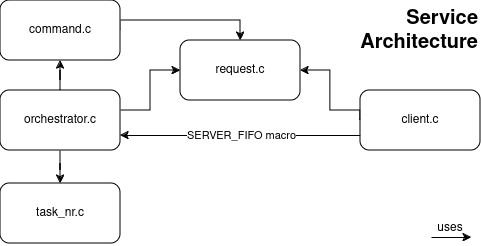
\includegraphics[scale=0.7]{diagrams/architecture.png}
            \caption{Arquitetura do Serviço}
            \label{fig:1.1}
        \end{figure}
    \section{Descrição dos Módulos Desenvolvidos}
        \subsection{Orquestrador (\textit{orchestrator.c})}
            O \textit{orchestrator.c} é o módulo principal do serviço, sendo responsável por:
            \begin{itemize}
                \item Leitura e validação dos argumentos da linha de comandos;
                \item Criar o seu \textit{FIFO} para receber pedidos dos clientes;
                \item Lidar adequadamente com os pedidos recebidos dos clientes;
                \item Caso o número máximo de tarefas em paralelo seja atingido,
                    colocar os pedidos de execução em espera;
                \item Caso necessário, enviar as respostas dos pedidos dos clientes pelos seus respetivos \textit{FIFOs}.
            \end{itemize}

            O orquestrador encarrega-se de quatro tipos de pedidos:
            \begin{itemize}
                \item \textit{\textbf{EXECUTE}} - Pedido para executar um comando.
                    Se o número máximo de tarefas em paralelo for atingido,
                    o orquestrador coloca o pedido em espera,
                    de seguida envia uma resposta ao cliente com o número da tarefa
                    e o estado do pedido ("a executar" ou "agendada").

                \item \textit{\textbf{COMPLETED}} - Assim que um comando terminar a sua execução,
                    o orquestrador recebe um pedido deste tipo enviado pelo processo-pai do processo-filho
                    que executou o comando, e executará, com base na política de escalonamento utilizada,
                    o próximo comando em espera, se algum existir.

                \item \textit{\textbf{STATUS}} - Pedido para consultar o estado das tarefas.
                    O orquestrador utiliza um processo para gerar e enviar a resposta ao cliente.
                    Deste modo, o servidor pode continuar a receber e lidar com pedidos de outros
                    clientes, sem interrupções.

                \item \textit{\textbf{KILL}} - Pedido para terminar o servidor.
                    Quando o orquestrador recebe este pedido,
                    termina a sua execução, porém, antes de terminar,
                    guarda o número de tarefa atual,
                    fecha os descritores de \textit{FIFOs} abertos,
                    e liberta a memória alocada para as tarefas em execução e em espera.
            \end{itemize}
            O orquestrador continua a correr até receber o pedido \textit{kill} de um cliente,
            ou até receber um sinal do sistema operativo para interromper/terminar.

            Para uma ilustração mais detalhada da comunicação entre o servidor e o cliente,
            por favor consulte os seguinte diagramas de comunicação nas figuras
            \textit{\ref{fig:1.2}} e \textit{\ref{fig:1.3}}, do subcapítulo \textit{\nameref{sec:1.3}}.

        \subsection{Cliente (\textit{client.c})}
            O módulo \textit{client.c} é responsável por, após a leitura e validação dos argumentos da linha de comandos,
            enviar pedidos - \textit{execute}, \textit{status} e \textit{kill} - para o \textit{FIFO} do
            servidor \textit{orchestrator}, e por receber as respostas do servidor num \textit{FIFO} criado para o efeito,
            no caso do pedido enviado ser do tipo \textit{execute} ou \textit{status}. O nome do \textit{FIFO} do cliente
            é gerado através do seu PID, e é enviado no próprio pedido para o servidor.
        \subsection{Pedido (\textit{request.c})}
            Neste módulo, é definida a estrutura de dados que representa um pedido, constituída por:
            \begin{itemize}
                \item \textbf{\textit{int type}} - Tipo do pedido
                    (\textit{EXECUTE}, \textit{COMPLETED}, \textit{STATUS} ou \textit{KILL});
                \item \textbf{\textit{int est\_time}} - Tempo estimado de execução da tarefa
                    ou a prioridade da tarefa, dependendo da política de escalonamento;
                \item \textbf{\textit{char command[MAX\_CMD\_SIZE]}} - Comando a executar, caso seja um pedido de execução;
                \item \textbf{\textit{bool is\_piped}} - Indica se o comando é encadeado, caso seja um pedido de execução;
                \item \textbf{\textit{unsigned int task\_nr}} - Número da tarefa, atribuído pelo orquestrador, caso seja um pedido de execução;
                \item \textbf{\textit{char client\_fifo[CLIENT\_FIFO\_SIZE]}} - Nome do \textit{FIFO} do cliente,
                    para onde o orquestrador enviará a resposta, caso seja um pedido de execução ou de estado.
            \end{itemize}

            Este módulo exibe garante o encapsulamento de dados, este é garantido através da definição da
            \textit{struct request} dentro do ficheiro \textit{request.c}, e a sua manipulação é feita através
            de funções definidas neste módulo, como por exemplo a função \textit{create\_request}, e as funções
            de \textit{getters} e de \textit{setters}.

            Também a oferece outra funções de utlidade, como a função de clonagem de pedidos, e impressão de pedidos,
            utlizadas no orquestrador.

        \subsection{Comando (\textit{command.c})}
            O módulo \textit{command.c} é chamado pelo orquestrador para executar os comandos enviados pelos clientes.

            Este módulo é responsável por:
            \begin{itemize}
                \item Executar comandos, \textit{single} ou \textit{piped}, utilizando \textit{process forking},
                    fazendo o respetivo \textit{parsing} dos comandos;
                \item Lida com o redirecionamento do \textit{stdout} e \textit{stderr} para os respetivos ficheiros;
                \item Encarrega-se da a escrita do tempo de espera mais o de execução das tarefas para ficheiro;
                \item Escreve o número da tarefa, o comando executado e o tempo total para o ficheiro de histórico.
            \end{itemize}

            Primeiramente, todos os ficheiros necessários são criados - nomeadamente a diretoria de
            \textit{output} para os ficheiros relativos a tarefa, como o ficheiro de \textit{output},
            o de erros e o do tempo total.
            Também prepara a abertura do ficheiro de histórico, onde serão escritos os dados como o número da tarefa,
            o comando executado e o tempo total, após a execução do comando.

            De seguida, é criado um processo utilizado para criar outro processo-filho que executará o comando.
            O processo-pai aguardará que o seu processo-filho termine a execução do comando, e, após a sua execução,
            escreverá o número da tarefa, o comando executado e o tempo total, em milissegundos, para o ficheiro de histórico,
            e notifica o orquestrador que a tarefa foi concluída.

            São criados dois processos para que o processo-pai interior possa esperar pela execução do comando,
            sem bloquear a execução do orquestrador, permitindo a este continuar a lidar com outros pedidos de clientes.

            O redirecionamento do \textit{stdout} e \textit{stderr} para os respetivos ficheiros é feito
            através da utilização da função \textit{dup2}.

            No encadeamento de comandos, o redirecionamento é feito de forma a que o \textit{stdout} do comando
            anterior seja redirecionado para o \textit{stdin} do comando seguinte, e assim sucessivamente. Ao longo
            da cadeia de comandos é feito o redirecionamento do \textit{stderr} para o ficheiro de erros, garantindo
            a similaridade com o comportamento nativo da \textit{shell}. No último comando, o redirecionamento do
            \textit{stdout} é feito para o ficheiro de \textit{output}.

        \subsection{Número de Tarefa (\textit{task\_nr.c})}
            O módulo \textit{task\_nr.c} proporciona funções para salvar e carregar o número
            de tarefa do respetiivo ficheiro com a designação definida pela
            \textit{macro TASK\_NR\_FILENAME}, neste caso, "task number".

            Se, ao carregar o ficheiro do número da tarefa, este não existir,
            o número da tarefa é inicializado a 1,
            caso contrário, o número da tarefa é incrementado em 1.

            Este módulo é utilizado pelo orquestrador na sua inicialização para carregar o
            número da tarefa, e no seu término para o salvar.

    \clearpage
    \section{Diagramas de Comunicação entre Servidor e Cliente}
        \label{sec:1.3}
        Nos seguintes três subcapítulos, são apresentados diagramas que ilustram a comunicação
        entre o servidor e o cliente, consuante diferentes tipos de pedidos.
        \subsection{Execução de Tarefas (\textit{execute})}
                \begin{figure}[!ht]
                    \centering
                    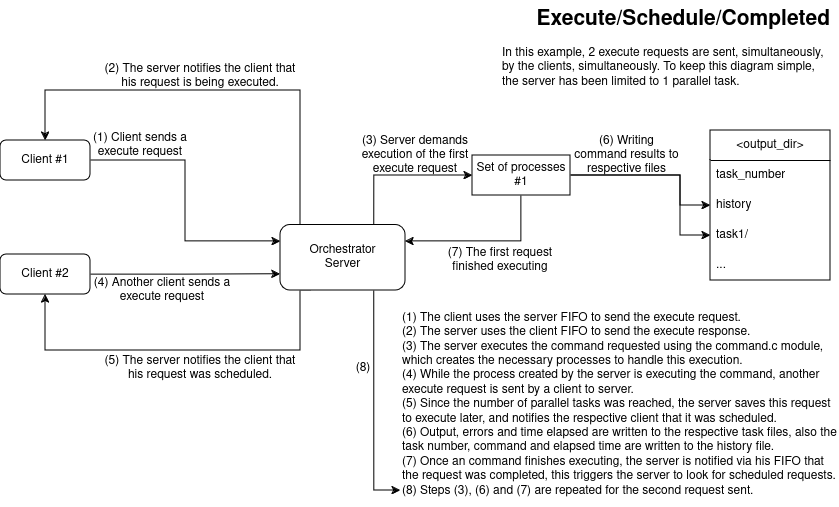
\includegraphics[width=\textwidth]{diagrams/execute.png}
                    \caption{Diagrama de Comunicação para Execução de Tarefas}
                    \label{fig:1.2}
                \end{figure}
        \subsection{Estado de Tarefas (\textit{status})}
            \begin{figure}[!ht]
                \centering
                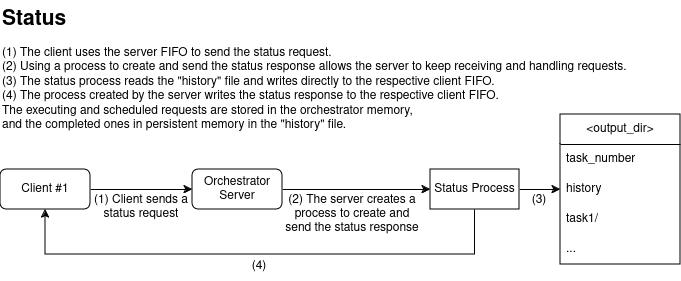
\includegraphics[width=\textwidth]{diagrams/status.png}
                \caption{Diagrama de Comunicação para Estado de Tarefas}
                \label{fig:1.3}
            \end{figure}
        \subsection{Terminação do Servidor (\textit{kill})}
            Na terminação do servidor, o cliente envia um pedido \textit{kill} para o \textit{FIFO} do servidor.
            De seguida o servidor guarda o número atual da tarefa de forma persistente,
            fecha os descritores de \textit{FIFOs} abertos,
            liberta a memória alocada para as tarefas em execução e em espera, e, por fim, termina a
            sua execução.

\begin{minipage}{\textwidth}
\chapter{Argumentos da Interface de Linha de Comandos}
    \section{\textit{Orchestrator}}
\begin{lstlisting}
Usage: orchestrator <output_dir> <parallel_tasks> [sched_policy]

Options:
    <output_dir>         Directory to store task output and history files
    <parallel_tasks>     Maximum number of tasks running in parallel
    [sched_policy]       Scheduling policy (FCFS, SJF, PES) default: SJF
\end{lstlisting}
    \section{\textit{Client}}
\begin{lstlisting}
Usage: client <option [args]>

Options:
    execute <est_time|priority> <-u|-p> "<command [args]>"            Execute a command
        est_time    Estimated time of execution, in case scheduling policy is SJF
        priority    Priority of the task, in case scheduling policy is PES
        -u          Unpiped command
        -p          Piped command
        command     Command to execute. Maximum size: 300 bytes
    status                                                            Status of the tasks
    kill                                                              Terminate the server

Note: The estimated time or priority is irrelevant if the scheduling policy is FCFS, but it must be provided as an argument.
\end{lstlisting}
\end{minipage}

\chapter{Avaliação de Políticas de Escalonamento}
    No trabalho desenvolvido, foram implementadas três políticas de escalonamento de tarefas.
    Estas serão aprofundadas nas secções seguintes, assim como as suas avaliações práticas.
    Por favor consulte o anexo \nameref{anexo:2} para mais detalhes de como foi realizada
    a implementação destas políticas.

    \textcolor{red}{>> Atualizar a introdução da avaliação de políticas de escalonamento.}
    \section{\textbf{FCFS} - \textit{First Come First Served}}
        Nesta política, as tarefas são executadas por ordem de chegada, o que não é
        eficiente em termos de tempo de espera e execução. No entanto, é uma política
        simples e fácil de implementar.

        \textcolor{red}{>> Escrever sobre a avaliação prática desta política + Imagem}
    \section{\textbf{SJF} - \textit{Shortest Job First}}
        A política \textit{Shortest Job First} é uma política de escalonamento não preemptiva
        que seleciona a tarefa com o menor tempo de execução. Este tempo é passado como
        argumento na opção \textit{execute} do cliente e repesenta uma estimativa do tempo
        que a tarefa demorará a ser executada.

        Esta política é eficiente em termos de tempo de espera e execução, mas pode levar
        a situações de \textit{starvation}, que ocorrem quando tarefas com tempos de execução
        maiores são sempre adiadas, e, num caso extremo, quando surgem constantemente tarefas
        com tempos de execução menores, estas de maior duração nunca serão executadas.

        Existem várias maneiras de lidar com situações de \textit{starvation}, como, por exemplo,
        a criação de uma especificação de tempo máximo de espera para cada tarefa, ou a
        definição de um número máximo de tarefas que podem ser executadas antes de uma
        tarefa com tempo de execução maior. Outra solução seria a implementação de uma
        política de escalonamento preemptiva, permitindo esta a interrupção de tarefas em
        execução para dar lugar a tarefas com tempos de execução menores.

        \textcolor{red}{>> Escrever sobre a avaliação prática desta política + Imagem}
    \section{\textbf{PES} - \textit{Priority Escalonation Scheduling}}
        De forma a evitar situações de \textit{starvation}, foi implementada a política
        \textit{Priority Escalonation Scheduling}. Nesta, as tarefas são executadas
        de acordo com a sua prioridade, que é definida pelo cliente na opção \textit{execute},
        simliarmente como o tempo estimado que é passado como argumento na política \textit{SJF}.

        As tarefas com maior prioridade são executadas primeiro, evitando
        situações de \textit{starvation}. As prioridades ficam a critério do cliente,
        possibilitando uma maior versatilidade na execução de tarefas, permitindo ao cliente
        definir a prioridade adequada para cada tarefa que deseja executar. No entanto, esta
        flexibilidade não garante a eficiência da execução das tarefas, caso estas não sejam
        corretamente priorizadas.

        \textcolor{red}{>> Escrever sobre a avaliação prática desta política + Imagem}

\chapter{Testes Desenvolvidos}

%==========================================================================
% BEGIN CONCLUSÃO
%==========================================================================

\chapter{Conclusão}
    Após o desenvolvimento deste serviço, foram cumpridos todos
    os objetivos propostos no enunciado do trabalho, desde a implementação de
    uma interface de linha de comandos tanto para o servidor como para o cliente -
    que permite a execução de tarefas do utilizador de forma assíncrona com a
    possibilidade de encadeamento de programas com \textit{pipes} e a
    consulta do estado das tarefas -, assim como a implementação de um ficheiro
    \textit{log} para guardar as tarefas executadas, bem como a implementação de um
    sistema com várias políticas de escalonamento e a avaliação prática destas.
    Também foi desenvolvido um conjunto de testes que permitem verificar o correto
    funcionamento do serviço.

    Após a afirmação da possibilidade da terminação ou interrupção do servidor
    pelo professor regente, foi despertada a curiosidade de como o servidor
    poderia lidar com estas situações.

    Num estudo apronfundado desta unidade curricular, uma solução seria a
    implementação de um sistema de interrupções no servidor, o que permitiria
    a este lidar com situações de terminação ou interrupção de forma mais
    eficiente através da utlização dos sinais do sistema operativo para lidar com estas
    situações, evitando a perda de tarefas agendadas ou em execução.

    Para tal, seria necessário lidar com tarefas em execução, guardando
    o estado destas em memória, e permitindo a sua correta terminação
    ou interrupção, assim como para as tarefas em espera. Estas poderiam
    ser guardadas numa fila de espera, que seria consultada sempre que
    uma tarefa terminasse, permitindo a execução da próxima tarefa na
    fila.

    Em suma, o desenvolvimento deste serviço permitiu a aplicação prática
    dos conhecimentos adquiridos ao longo do semestre, assim como a
    exploração de novas funcionalidades e conceitos, que proporcionaram
    a implementação de um serviço robusto e versátil - serviço este que 
    propicia a execução de tarefas de forma assíncrona, com a possibilidade de
    encadeamento de programas e a consulta do estado das tarefas.

%==========================================================================
% END CONCLUSÃO
%==========================================================================

%==========================================================================
% BEGIN ANEXOS
%==========================================================================
%
%% Why \addchap, instead of \chapter?
%% \addchap has no numbering but appears in table of contents.
\addchap{Anexos}

    \addsec{
        \href{anexos/refman.pdf}{\small \textcolor{blue}{[I] Documentação do Código Desenvolvido}}
        \label{anexo:1}
    }

    \quad Para uma versão mais interativa da documentação do código desenvolvido, por favor consulte o
    ficheiro \textbf{\textit{doc/html/index.html}} localizado na diretoria raiz do projeto com o seu
    navegador de internet.

    \addsec{
        \href{anexos/example.pdf}{\small \textcolor{blue}{[II] Implementação das Políticas de Escalonamento}}
        \label{anexo:2}
    }

%==========================================================================
% END ANEXOS
%==========================================================================
\end{document}
